\documentclass[a4paper,oneside]{article}

  \usepackage{graphicx}
  \usepackage{subcaption}
  \usepackage{xcolor}
  \usepackage{hyperref}
  \usepackage[cm]{fullpage}
  \usepackage{booktabs}
  \usepackage{lmodern} 
  \usepackage[T1]{fontenc}
  \usepackage{amsmath}

\begin{document}
  \section*{The hypothetical adaptive value of the generalized growth arrest and the constraints for a successful sex event}
    Molecular, biophysical and chemical data discussed above unequivocally show that \textit{P.~multistriata}, during events of mating and gametogenesis, blocks growth and mitosis for a few days --- three in the experiment discussed here, and up to six in the one discussed by Scalco et al. (2014).
    Also, cell number decreases, very likely for enhanced mortality due to the gametogenesis.
    To analyze the impact of such behaviour on population dynamics, we developed a simple process-based model of growth dynamics during the sexual reproduction event, where net growth is the balance between size-dependent cell growth and death.
    The model is conceptually zero-dimensional, and the initial conditions consider the minimal cell concentration recorded by Scalco et al. (2014) as gametogenesis trigger.
    Cell numbers and available Nitrogen are expressed as abundance and concentration, respectively.

    The simulation starts with a cell population ($P$) that enters the sexual reproduction phase after reaching a threshold value of a few thousand cells per ml (see Scalco et al., 2014).
    During this phase of variable length, the population stop growing and experience a prolonged burst of extra mortality.
    Within the same span, a $P$ fraction will undergo gametogenesis and generate an offspring population ($F_{1}$) that will start to grow the moment ($t_{F_{1}I}$) it appears.
    After $t_{AE}$ days, the growth arrest will end and $P$ will resumes its growth alongside $F_{1}$.
    During the entire course of the simulation (set to ten days) cell growth is modulated by competition over Nitrogen and by cell size via an allometric relationship (see m'Alelio et al., 2010).

    A fundamental assumption, discussed later in the text, is that parental and daughters cells share a common, exclusive space, so that only $P$ and $F_{1}$ compete for N made available in such space.
    This assumption is translated in the model as a decrease in growth rate as the total population ($F_{1} + P$) converges toward the carrying capacity, set as the total nitrogen content of initial parental cells.

    To understand better how event timing and response amplitudes impact over $F_{1}$ recruitment success, we compared simulation outputs across selected parameters range.
    Our selected parameters are the $P$ fraction that will generate $F_{1}$ ($\alpha$), gametogenesis-induced extra mortality of parental cells ($m$), duration of the growth arrest ($t_{AE}$), and growth rates ratio among parental and initial cells ($r_{P}:r_{F_{1}}$)
    We deployed an interactive version of the model at the URL \url{https://arfalas.shinyapps.io/pns_toy/}, code and figures are available on \url{https://github.com/bhym/Stec} ({\color{red} currently private})
%
  \section*{Model description}
    Parental ($P$) and offspring ($F_{1}$) dynamics are defined as ODE:\@
    %
    \begin{align}
      \frac{dP}{dt}     &= \kappa \mu_{P} P - \delta P \\
      \frac{dF_{1}}{dt} &= \kappa \mu_{F_{1}} F_{1}
    \end{align}
    %
    where $\kappa$ is the competition for N, defined as
    \[
      1 - \frac{{[N]}_{t}}{1.2{[N]}_{t=0}}
    \]
    with 
    \[
      [N_{t}] = {[P]}_{t} {[N]}_{P} + {[F_{1}]}_{t} {[N]}_{F_{1}}
    \]

    $\mu_{P}$ and $\mu_{F_{1}}$ are defined as
    \[
      \mu_{P} =
        \begin{cases}
          0                    & \mbox{if } t <    t_{AE} \\
          \lambda_{P}(t) r_{P} & \mbox{if } t \geq t_{AE}
        \end{cases}
      \qquad;\qquad
      \mu_{F_{1}} = 
        \begin{cases}
          0                            & \mbox{if } t <    t_{F_{1}I} \\
          \lambda_{F_{1}}(t) r_{F_{1}} & \mbox{if } t \geq t_{F_{1}I}
        \end{cases}
    \]
    with $\lambda_i(t)$ representing allometric scaling on length ($L$), defined as
    \[
      \lambda_{i}(t) = 0.25 + 0.04 L_{i}(t) - 0.0005 L_{i}{(t)}^{2}
    \]
    Length dynamics are based on cell's age ($a$) and are defined by the rule
    \[
      L_{i}(t) = L_{0,i} - 0.1 a(t) \hspace{8mm}\text{with $i$ either $P$ or $F_{1}$}
    \]
    Age is counted from the appearance of the population, and does not increase during GA.\@

    Finally, $\delta$ is an extra mortality term defined as
    \[
      \begin{cases}
        m & \mbox{if } t < t_{AE} \\
        0 & \mbox{if } t > t_{AE}
      \end{cases}
    \]
    The parameters values and ranges are reported in \textbf{Table~\ref{tbl1}}.
    %
    \begin{table}
      \centering
      {%
        \begin{tabular}{@{}llccr@{}}
          \toprule
          \textbf{Variable}&\textbf{Meaning} & \textbf{Units} & \textbf{Value} & \textbf{Reference}\\
          \midrule
          ${P}_{0}$       & initial concentration of $P$ cells         & cells/ml          & 4E3         & Experiment detailed in the paper\\
          $\alpha$        & fraction of $P$ that will generate $F_{1}$ & ---               & [0.01, 0.2] & Explored via simulations\\
          $r_{P}$         & net growth rate of $P$                     & $\text{day}^{-1}$ & [0.5, 3]      & Explored via simulations\\ 
          $r_{F_{1}}$     & net growth rate of $F_{1}$                 & $\text{day}^{-1}$ & 1           & ---\\
          $t_{AE}$        & end day of the growth arrest               & day               & [2,6]       & Explored via simulations\\
          $t_{F_{1}I}$    & day of appearence of the offspring         & day               & 3           & Experiment detailed in the paper\\
          $L_{0,P}$       & starting length for $P$ cells              & $\mu$m            & 40          & Experiment detailed in the paper\\
          $L_{0,{F_{1}}}$ & starting length for $F_{1}$ cells          & $\mu$m            & 80          & Experiment detailed in the paper\\
          $m$             & gametogenesis-induced extra mortality      & day               & [0.1, 0.9]  & Explored via simulations\\
          \bottomrule
        \end{tabular}
       }
      \caption{Values and ranges for model parameters}\label{tbl1}
    \end{table}
%
  \section*{Results and Discussion of the simulations}
    \textbf{Fig.~\ref{fdyn}} shows the relative variation of allometric growth (\textbf{plot {\color{blue}\textit{a}}}) as derived from the equation reported above.
    Considering the time interval chosen for the simulation (ten days), the size reduction of $P$ and $F_{1}$ (\textbf{plot {\color{blue}\textit{b}}}) is negligible and, with it, the change in the growth rate of $P$ and $F_{1}$, with a significantly slower growth rate for $F_{1}$ due to their larger size.
    \textbf{Plots {\color{blue}\textit{c}}} and {\textbf{\color{blue}{\textit{d}}}} show the variation in abundance of $P$ and $F_{1}$ for two different sets of parameters used for the simulation.
    These plots provide a demonstration of the dynamics that the model simulates.
    A slower growth rate of $P$ ($r_p=1$, \textbf{plot {\color{blue}\textit{d}}} vs $r_p=1.82$, \textbf{plot {\color{blue}\textit{c}}}) that leaves more nitrogen available favours the growth of $F_{1}$, thus producing a greater abundance of $F_{1}$ and a lower abundance of $P$.

    The ten days length for growth arrest was chosen arbitrarily as a realistic time interval during which parental and daughter cells could remain close one to the other in a low sheared flow regime, so that the hypothesis of resources sharing could hold.
    The time spent in close vicinity by cells in a viscous regime  --- as the one we found in situ --- has been seldom analyzed in detail (see Jenkinson \& Wyatt, 1992 [Journal of Plankton Research, 14:1697--1721]).
    However, we assume that to permit mating, which implies direct contact among mates, several cells should converge by some mechanism --- for example, the one hypothesized by Botte et al., 2013 [J. Plankton Research 35: 914--918] and recently supported with observations by Font-Mu{\~n}oz et al.~(2019) [PNAS 116:15997--16002].
    On the basis of this assumtpion, our scenario would simulate local aggregations of cells, whose reproduction is favoured by the reaching of what we define threshold density.
    This concentration should be enough to trigger gametogenesis by chemical signal exchange ({\color{green}\textbf{ref}}).
    Once the gametogenesis starts all the involved cells stop growing and some individuals will form gametes, likely because the triggering caugth them in a specific phase of the cell cycle.
    Only a part of these gametes will encounter the opposite mating type, and only some of these will successfully complete the other phases,producing an $F_{1}$ generation (e.g., Scalco et al.~2014).
    Eventually, those unable to mate or complete gametogenesis will die.
    These considerations are compatible with the observed negative growth rate of $P$, and are formulated in the model as extra mortality ($m$).

    Assuming that auxospore formation scales with the encounter rate among mates, the number of auxospore formation should positively covary with the number of cell deaths due to unsuccessful encounters.
    This covariation would favour the $F_{1}$ growth, thus favouring better recruitment.
    Also, more encounters will increase the number of successful matings (parametrised by $\alpha$) and the extra mortality (parametrised by $m$).
    In the following we discuss the main patterns resulting from simulations where the different parameters were varied, in all possible combinations, within the ranges reported in \textbf{Tab.}~\ref{tbl1}
    As the main output variable, we focused on the recruitment success of the offsprings --- quantified as the ratio between $F_{1}$ and $P$ ($r_p : r_{F_{1}}$) --- after ten days from the start of mating.

    Top row in \textbf{Fig.}~\ref{swep} show the ratio between the abundance of $F_{1}$ and that of $P$ after ten days of simulation for the growth rates ratio of $F_{1}$ and $P$ ($r_P : r_{F_{1}}$ on the $Y$ axis) vs $m$, the extra mortality ($X$ axis).
    The colours correspond to different ranges in the values of the decimal logarithm for the abundance ratio, e.g., $\log_{10}(F_{1}/P)$ and each plot displays the result for different durations of the growth arrest ($t_{AE}$).
    While $F_{1}$ will always be lower than $P$ (values of $\log_{10}(F_{1}/P)$ always lower than $0$), if the arrest persist more than four days a positive feedback appears between  abundance ratio and both net growth rates ($r_P : r_{F_{1}}$) and extra mortality $m$.
    In the more favourable scenarios, the ratio in abundance among $F_{1}$ and $P$ would be larger than $0.17$ (6 days of GA, dark green areas on the lower left).
    The lower row of the same figure shows the log-ratio among $F_{1}$ and $P$ abundances for various growth rate ration ($r_P : r_{F_{1}}$ on the $Y$ axis) vs the fraction of parental cells that generated daughter cells $F_{1}$ ($\alpha$), through auxospore formation.
    Success in recruitment appears to increase $F_{1}$ success, while growth rate ratio seems to affect it only for longer duration of growth arrest.

    We report the values of $\log_{10}(F_{1}/P)$ for different combinations of the parameters as supplementary tables \textbf{Table~\ref{tbl2}}..
    Overall the simulation provides a quantitative assessment of the number of $F_{1}$ that accumulate after ten day from the start of gametogenesis in relation to the number of mating cells and show that:
    1.\ only in extreme scenarios $F_{1}$ abundance will be equal or higher than $P$ and
    2.\ that the biological constrains of gametogenesis (growth arrest and extra death) due to resetting of cell physiology are compensated by an advantage for the $F_{1}$, mimicking a sort of maternal care.

    The constraints imposed by the series of events leading to \textit{Pm} recruitment also suggest that blooming is advantageous because increase the number of initial cells, thus allowing for a better seeding of the community with the new generation.
    Furtmermore, the concentration increase during bloom has a strong positive feedback on mating --- itself scaling with parental cell abundance, related to $\alpha$ in the model --- because it boost encounter rate.
    D'Alelio et al. (2010) inferred form data and modeling that the life cycle of \textit{Pm} consists of two phases characterised by opposite growth rate trends (slow vs fast).
    The shift in rates is collective and appears during bloom events, during which cells prepare for sexual reproduction.
    Identifying the triggers of this collective process would shed light on the long lasting debate on the relative weight of proximate vs ultimate factors (10.1126/science.1210879) and on the main drivers of the population dynamics of several diatoms.

    Relaxing the assumption that all the nitrogen left unused by blocked parental cells or regenerated from their death is used by the daughters with the possibility that part of it would go to other species in the community would just decrease the recruitment success but would produce an advantage for the other species in the community.

    In SM, we report the impact on the structure of the community and species succession of a sexual reproduction event in a simulation with a biogeochemical model reproducing the conditions of a North Atlantic site.
    Diatom sex events may be one of the factors that affect phytoplankton succession and changes in community structure in nature.
    %
    \begin{figure}[p]
      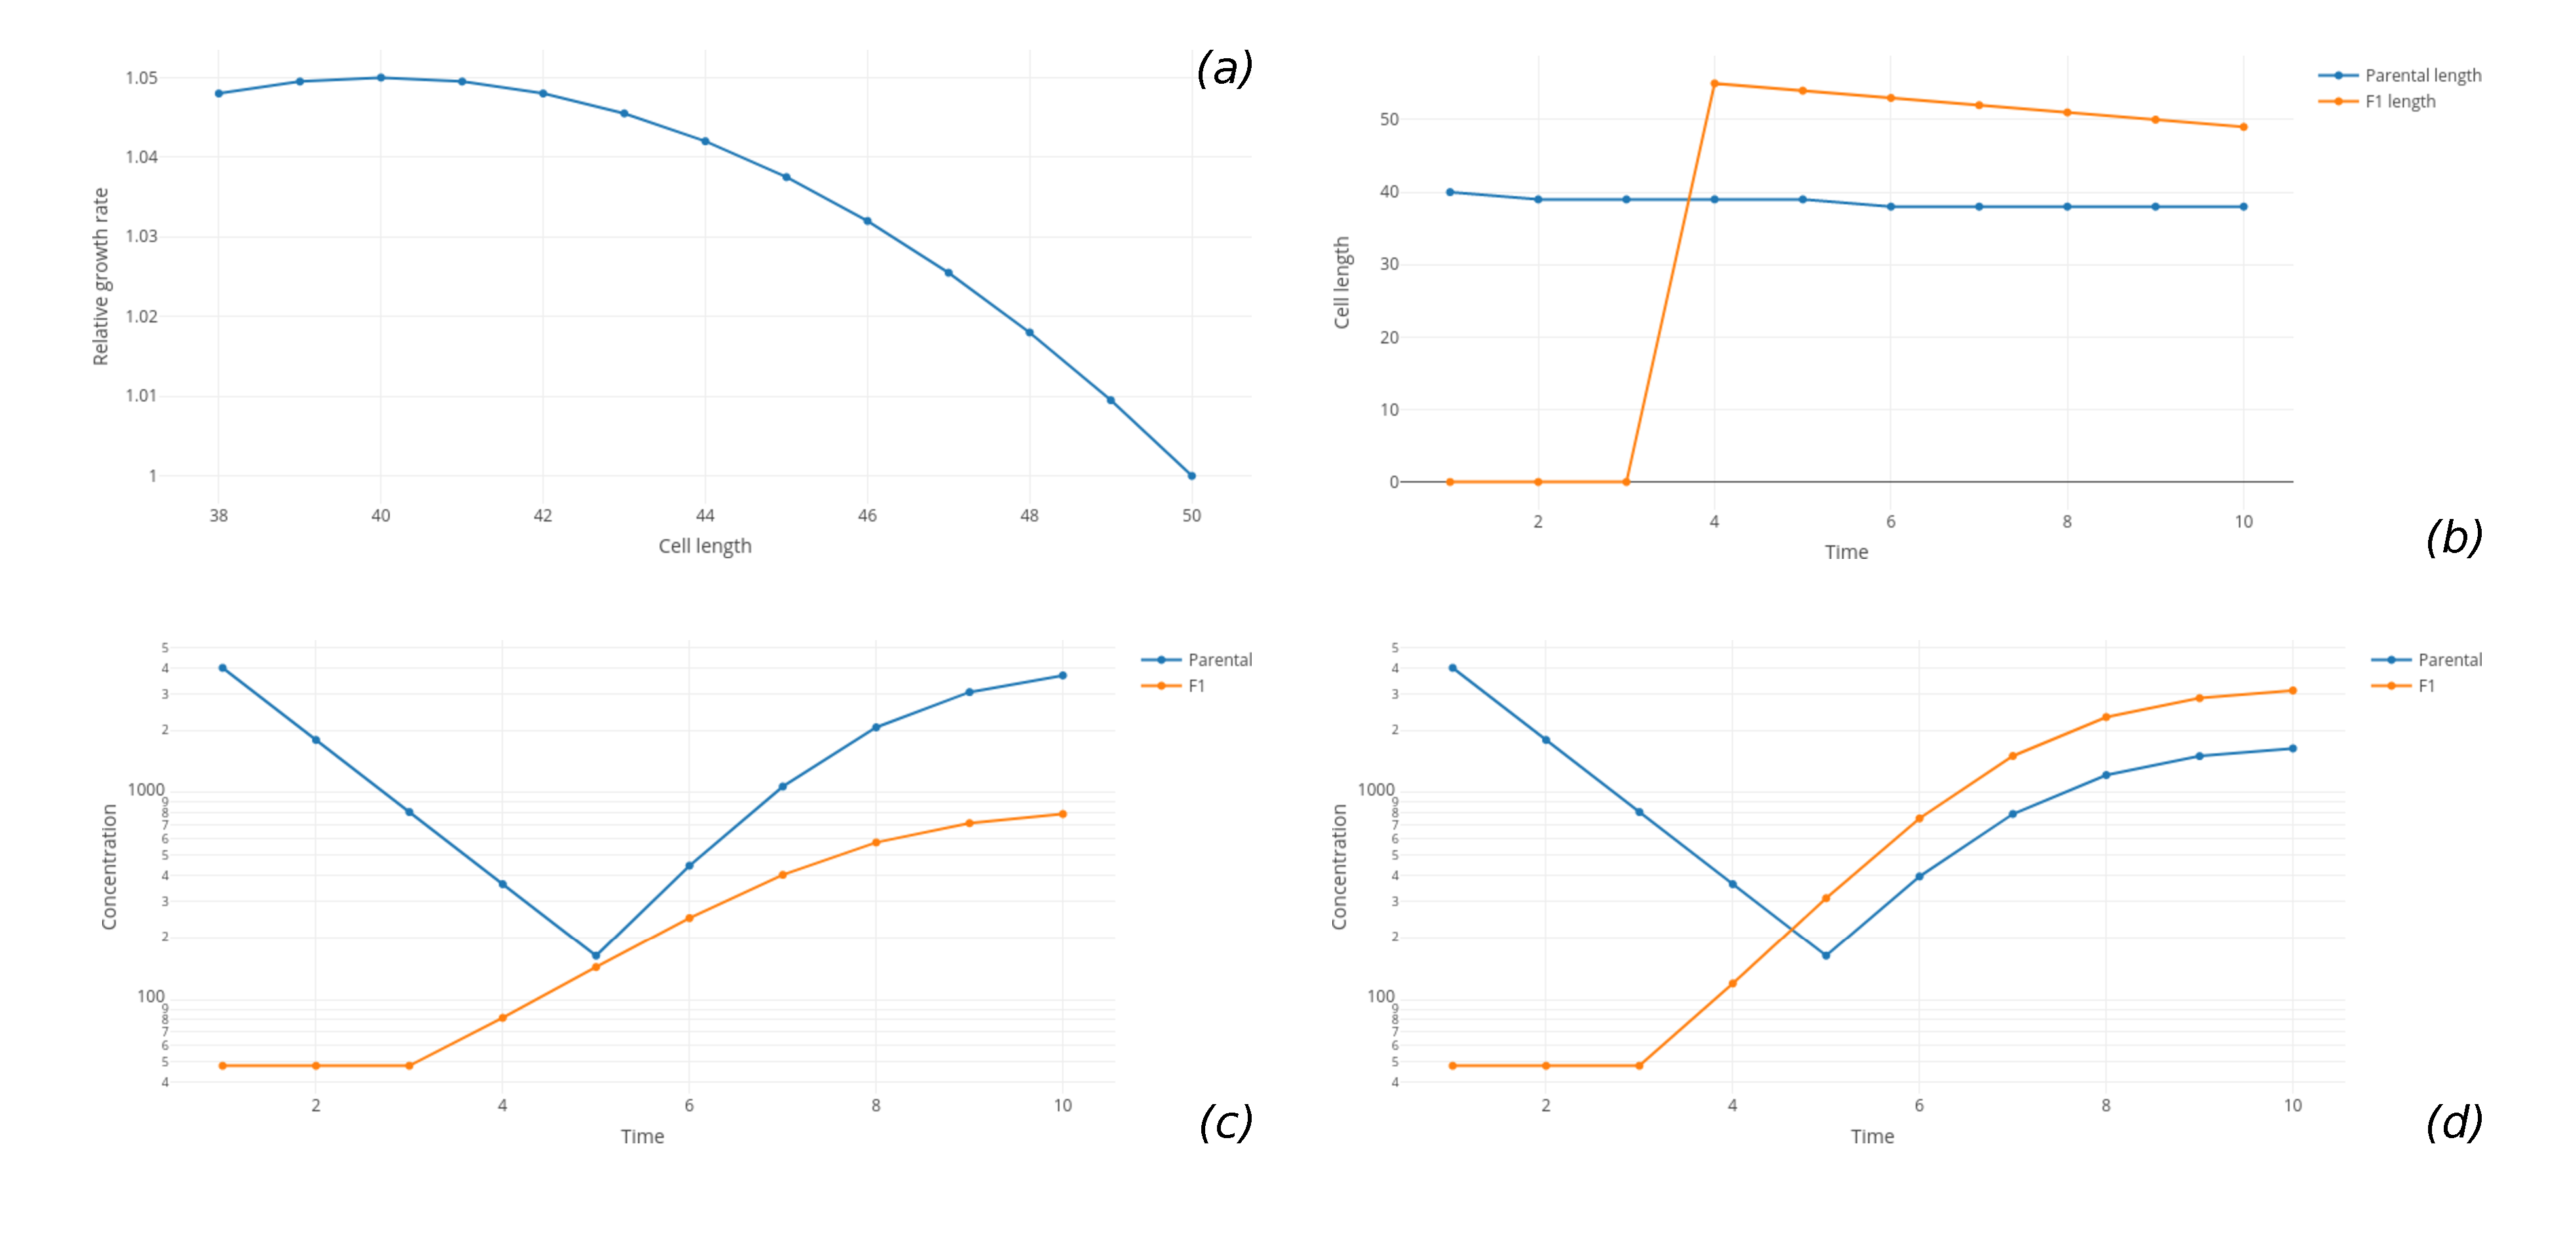
\includegraphics[width=\linewidth]{imgs/Figpan.pdf}
      \caption{\textbf{Simulated size dependent growth and impact on the population dynamics} ---
        {\color{blue}\textit{(a)}} dependence of specific growth rate on cell length;
        {\color{blue}\textit{(b)}} Size reduction for the two sub-populations;
        examples of simulation outputs whith $r_{p} >r_{f1}$ (1.06 and 0.58, respectively) {\color{blue}\textit{(c)}} and $r_{p} = r_{f1}$ {\color{blue}\textit{(d)}}.
        In {\color{blue}\textit{(c)}} and {\color{blue}\textit{(d)}}: $\alpha=0.012, m = 0.8$, all the other parameters as per \textbf{Tab.~\ref{tbl1}}.
      }\label{fdyn}.
    \end{figure}
    %
    \begin{figure}[p]
        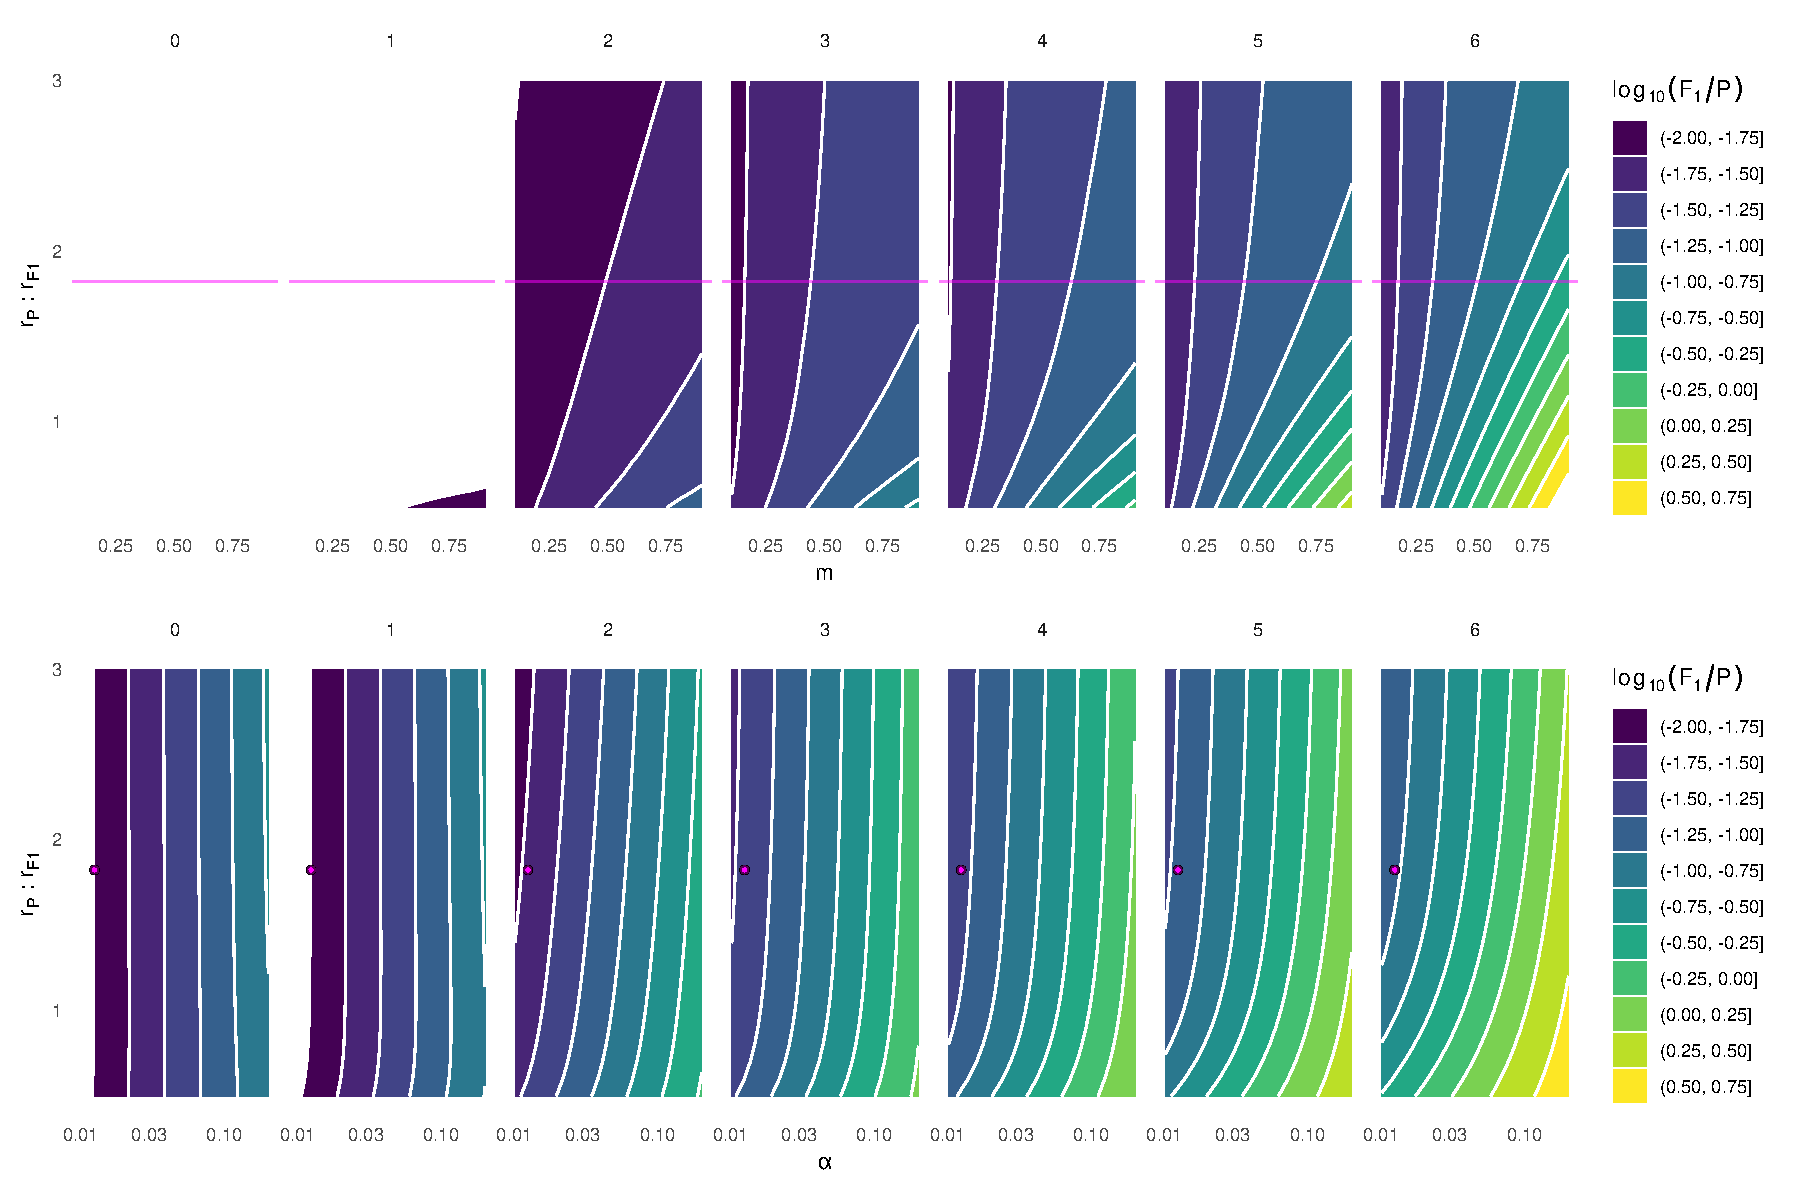
\includegraphics[width=\linewidth]{imgs/parswpan.pdf}
      \caption{\textbf{Contour plots of ranges of recruitment success after 10 days of simulation for paired values of parameters (axes labels).}
        Recruitment success is expressed as $\log_{10}(F_{1}/P)$; $\alpha$ is the fraction of $P$ cells that will generate $F_{1}$.
        Different subplots represent different durations of growth arrest ($t_{AE}$ model parameter).
        Parameters left unchanged during the simulations were assigned as per \textbf{Tab.~\ref{tbl1}}.
      }\label{swep}
    \end{figure}
    %
    \begin{table}[p]
      \centering
      {%
        \begin{subtable}{12cm}\centering\scriptsize
          {
\begin{tabular}{lrrrrrrrrr}
\toprule
  & 0.01 & 0.03 & 0.05 & 0.08 & 0.1 & 0.12 & 0.15 & 0.17 & 0.2\\
\midrule
3 & -1.72 & -1.23 & -1.00 & -0.79 & -0.68 & -0.59 & -0.48 & -0.42 & -0.34\\
2.7 & -1.71 & -1.23 & -1.00 & -0.78 & -0.68 & -0.59 & -0.48 & -0.42 & -0.34\\
2.5 & -1.71 & -1.23 & -1.00 & -0.78 & -0.68 & -0.59 & -0.48 & -0.42 & -0.34\\
2.2 & -1.71 & -1.22 & -0.99 & -0.78 & -0.67 & -0.59 & -0.48 & -0.42 & -0.33\\
2 & -1.70 & -1.22 & -0.99 & -0.77 & -0.67 & -0.58 & -0.47 & -0.41 & -0.33\\
\addlinespace
1.7 & -1.70 & -1.21 & -0.98 & -0.77 & -0.66 & -0.58 & -0.47 & -0.41 & -0.33\\
1.5 & -1.69 & -1.20 & -0.98 & -0.76 & -0.66 & -0.57 & -0.47 & -0.41 & -0.33\\
1.2 & -1.67 & -1.19 & -0.96 & -0.75 & -0.65 & -0.56 & -0.46 & -0.40 & -0.32\\
1 & -1.66 & -1.18 & -0.95 & -0.74 & -0.63 & -0.55 & -0.45 & -0.39 & -0.31\\
\bottomrule
\end{tabular}
}
          \caption{$\alpha, r_p:r_{f1}, \text{with } m = 0.2$}
        \end{subtable}
        \\
       \vspace{0.5cm}
        \begin{subtable}{12cm}\centering\scriptsize
          {
\begin{tabular}{lrrrrrrrrr}
\toprule
  & 0.01 & 0.03 & 0.05 & 0.08 & 0.1 & 0.12 & 0.15 & 0.17 & 0.2\\
\midrule
3 & -1.69 & -1.20 & -0.96 & -0.74 & -0.63 & -0.53 & -0.41 & -0.34 & -0.24\\
2.7 & -1.68 & -1.19 & -0.96 & -0.73 & -0.62 & -0.52 & -0.40 & -0.33 & -0.24\\
2.5 & -1.68 & -1.19 & -0.95 & -0.72 & -0.61 & -0.52 & -0.40 & -0.33 & -0.23\\
2.2 & -1.67 & -1.18 & -0.94 & -0.71 & -0.60 & -0.50 & -0.38 & -0.31 & -0.22\\
2 & -1.66 & -1.17 & -0.93 & -0.70 & -0.59 & -0.49 & -0.37 & -0.30 & -0.21\\
\addlinespace
1.7 & -1.64 & -1.15 & -0.91 & -0.68 & -0.57 & -0.47 & -0.35 & -0.28 & -0.19\\
1.5 & -1.62 & -1.13 & -0.89 & -0.67 & -0.55 & -0.46 & -0.33 & -0.26 & -0.17\\
1.2 & -1.59 & -1.09 & -0.86 & -0.63 & -0.51 & -0.42 & -0.29 & -0.22 & -0.13\\
1 & -1.55 & -1.05 & -0.81 & -0.58 & -0.47 & -0.37 & -0.25 & -0.18 & -0.09\\
\bottomrule
\end{tabular}
}
          \caption{$\alpha, r_p:r_{f1}, \text{with } m = 0.4$}
        \end{subtable}
        \\
       \vspace{0.5cm}
        \begin{subtable}{12cm}\centering\scriptsize
          {
\begin{tabular}{lrrrrrrrrr}
\toprule
  & 0.01 & 0.03 & 0.05 & 0.08 & 0.1 & 0.12 & 0.15 & 0.17 & 0.2\\
\midrule
3 & -0.92 & -0.42 & -0.18 & 0.05 & 0.16 & 0.25 & 0.36 & 0.41 & 0.49\\
2.7 & -0.87 & -0.37 & -0.13 & 0.10 & 0.20 & 0.29 & 0.40 & 0.45 & 0.53\\
2.5 & -0.84 & -0.34 & -0.09 & 0.13 & 0.24 & 0.32 & 0.43 & 0.48 & 0.55\\
2.2 & -0.78 & -0.27 & -0.03 & 0.19 & 0.30 & 0.38 & 0.48 & 0.53 & 0.60\\
2 & -0.72 & -0.22 & 0.02 & 0.24 & 0.34 & 0.42 & 0.52 & 0.57 & 0.63\\
\addlinespace
1.7 & -0.62 & -0.12 & 0.11 & 0.32 & 0.42 & 0.49 & 0.58 & 0.63 & 0.68\\
1.5 & -0.54 & -0.04 & 0.19 & 0.39 & 0.48 & 0.55 & 0.63 & 0.67 & 0.72\\
1.2 & -0.36 & 0.11 & 0.32 & 0.50 & 0.58 & 0.64 & 0.71 & 0.74 & 0.79\\
1 & -0.20 & 0.24 & 0.43 & 0.58 & 0.65 & 0.70 & 0.76 & 0.79 & 0.83\\
\bottomrule
\end{tabular}
}
          \caption{$\alpha, r_p:r_{f1}, \text{with } m = 0.6$}
        \end{subtable}
        \caption{Tabular data of $\log_{10}(F_{1}/P)$ for different values of parameters showed at bottom and growth arrest duration of three days.
                 All other parameters were assigned as per \textbf{Tab.~\ref{tbl1}}}\label{tbl2}
      }
    \end{table}
%
  \section*{Assumptions} 
    \begin{enumerate}
      \item I assume that net growth rate is the difference between size-dependent cell growth and death
      \item I assume that $P$ suffers extra mortality during growth arrest due to gametogenesis
      \item I assume that lenght decreases 0.1 um after each division
      \item I assume that $P$ has reached the environmental carrying capacity before starting the simulation
    \end{enumerate}
\end{document}
